\documentclass{article}
\usepackage{fancyref}
\usepackage{todonotes}
\usepackage[utf8]{inputenc}
\usepackage{pdfpages}

\usepackage[style=ieee,backend=biber]{biblatex}
\addbibresource{proposal-cites.bib}

\title{Project Proposal \\ Investigating strategies for agents to scam and to not get scammed on an abstract eBay}
\author{Christopher Taylor \\ Department of Computer Science \\ University of Bath \\ me@christophertaylor.net}

\begin{document}
\maketitle

\section{Problem Description}
\label{sec:problem-description}
There are many websites and services that facilitate trade between users, perhaps one of the best knowm being eBay. These services can be of great value to users for a wide variety of different purposes, but it can come at a cost - there are malicious users who attempt to defraud and scam others.

hese platform have several institutional methods of preventing fraud and reimbursing victims, but the feature that most factors into users' decision making is the feedback system. The feedback system gives buyers an opportunity to leave a comment and positive, negative or neutral feedback on a transaction. All of this information is made available to users when they are deciding to carry out a transaction - including a feedback score and the seller's percentage of positive feedback. From this, the potential buyer can decide whether or not they trust the user to not defraud them, and to deliver the goods in a good state, and in good time.\cite{gregg2006role}

The proposal is to create an abstract model of the eBay systems in order to explore some of the strategies users could employ on a service such as eBay. A simple model will be used to begin with, and more factors introduuced (\fref{sec:factors-strategies}) into agents' decision making processes - exploring factors in the model and in their wider academic context. Rather than just running each simulation once with a randomly generated set of agents, genetic algorithms will be employed in order to refine the strategies and parameters over many generations.

\subsection{The Model: Peer-to-Peer Trading Game}
\label{sec:P2PTG}
Each round of the \emph{Peer-to-Peer Trading Game} (henceforth referred to as \emph{P2PT Game or P2PTG}) will happen as follows:
\begin{itemize}
	\item N agents (representing users) are selected or generated using one of several possible methods.
	\item The of transactions, T, for the entire simulation is randomly determined, and hidden from the agents.
	\item T transactions run, each one going as follows:
	\begin{itemize}
		\item Two random agents from the list are selected.
		\item Each choose whether to Cooperate, Defect or Decline. An agent that chooses to cooperate goes into the transaction with good faith, while an agent that chooses to defect attempts to scam or cheat the other. Each agent also has the choice to decline a transaction. The payoff for these actions is defined in \fref{fig:model-payoff}.
		\item Each user then has the opportunity to leave feedback about the user they traded with (if the transaction actually went ahead - that is, if neither declined it).
	\end{itemize}
	\item After all the transactions, each agent's score is computed.
\end{itemize}

After each round of the game is complete, the results can be analysed and/or a new generation can be bred for the next round.
\begin{figure}[h]
	\begin{center}
		\label{fig:model-payoff}
		\caption{The Payoff Matrix for a Transaction}
		\begin{tabular}{| l || c | c | c |}
			\hline
			A1,A2 & A2 Cooperate & A2 Defect & A2 Decline \\ \hline
			A1 Cooperate & 2,2 & -2,4 & 0,0 \\ \hline  
			A1 Defect & 4,-2 & -1, -1 & 0,0 \\ \hline
			A1 Decline & 0,0 & 0,0 & 0,0 \\ \hline
		\end{tabular}
	\end{center}
\end{figure}

\subsection{Factors \& Strategies}
\label{sec:factors-strategies}
The project will start with a simple set of strategies and build increasingly complicated ones, drawing from research in a number of fields related to decision making.

The first iteration of the system will be very similar to the hawk-dove game\cite{smith1973lhe}. The most common formulation of the hawk-dove game is: two random birds from a population find a food resource at the same time. If both of the birds are doves, they share the food between them; if one is a hawk and the other is a dove, the dove retreats - leaving all the food to the hawk; if both are hawks, they fight for the resource (incurring the risk of injury, etc, in the process).

In terms of the P2PT game, the first version will contain two agents - those who always cooperate (doves) and those who always defect (hawks.) From there, the hawk and dove strategies will be enhanced with a range of possible different considerations:
\begin{description}
	\item[Basic Reputation/Feedback] - Doves will be able to see the reputation of the other user before deciding to trade with them or not - doves in this model will use the percentage of positive/negative feedback. To compensate, hawks will gain the ability to only defect a given percentage of the time.
	\item[Direct experience] - Humans act differently depending on \emph{who} the person is\cite{fehr2003nature}, rather than just their mathematical feedback. In this stage, agents will be able to take into account their direct experience with an agent. Each agent may weight it more or less than the other factors.
	\item[Whitewashing and number of transactions] - Whitewashing\cite{hoffman2009survey} is one of the types of attacks on reputation systems, by which a malicious user uses some method of clearing or altering their reputation. In terms of online auction sites, one way of doing this would be to start a new account (thus wiping the slate clean). For some utility cost, hawks will be able to reset their reputation values to 0. As a countermeasure, doves will be able to take into account the length of their opponent's reputation, not just the percent positive - weighting more consistent, lengthier records over shorter ones.
	\item[Lies and Slander] - Agents are no longer obligated to leave true feedback. Hawks will be able to slander\cite{hoffman2009survey} the doves they exploit (by leaving negative feedback when they chose to cooperate) and/or leave positive feedback for other hawks.
\end{description}

Each stage will examine in detail the issues to be considered, drawing from experimental results from the system and appropriate literature.

\section{Requirements Specification}
\label{sec:requirements-spec}
\subsection{Requirements for Report \& Platform}
\begin{enumerate}
	\item Develop a simulation platform for the Peer-to-Peer Trading game.
	\begin{enumerate}
		\item The platform should provide the framework for the implementation of a wide variety of agent strategies.
		\item The platform should provide some method of extracting useful data from the simulations for analysis.
	\end{enumerate}
	\item Use the platform to experiment with a number of different strategies and factors (as discussed in \fref{sec:factors-strategies}).
	\begin{enumerate}
		\item Bring together research and analysis of results from the P2PT game in order to comment on strategies in the initial scenario.
	\end{enumerate}
\end{enumerate}

\subsection{Non-functional Requirements}
\label{sec:non-functional}
\begin{enumerate}
	\item The platform and analysis tools to be written should be implemented using Python, version 3.4.
	\item The platform and analysis tools should be capable of running on a medium-range laptop (6GB RAM, 2.0GHz Quad Core) in under 12 hours per simulation.
	\item A limited number of larger, more intensive, experiments can be run on a higher-end desktop (20GB RAM, 2.8GHz Quad Core) in under 12 hours per simulation.
\end{enumerate}

\newpage
\section{Project Plan}
\label{sec:project-plan}
The deliverables for the project are:
\begin{description}
	\item[Project Proposal] - 27th October 2014
	\item[Literature and Technology Survey] - 21st November 2014
	\item[Demonstration of Progress] - 16th February 2015
	\item[Dissertation] - 1st May 2015
\end{description}

The timescale and composition of these tasks is shown on the next page. A number of considerations went into the plan at each deliverable milestone.
\begin{description}
	\item[Project Proposal] - The prototyping and writing of the proposal are concurrent activities, both informed by each other. Drafts of the proposal were written, then adapted with knowledge gained from early prototyping.
	\item[Literature and Technology Survey] - The time for the Literature Review is split roughly into two halves: one for taking the information in and making notes, the other for actually producing the literature review. Mostly completing the reading stage before first drafting the review itself should make planning and outlining the review an easier task, without having to allow for much in the way of later additions.
	\item[Demonstration of Progress] - The demonstration of progress itself is only a short presentation, which should take very little in the way of preparation time. The initial literature and experimentation phases of the project will have been completed by the time of the presentation, meaning that there will be something to present.
	\item[Disseration] - The dissertation has been divided into four sections: further literature compilation, programming/experimentation, compilation and writing, and miscellaneous tasks. The first two tasks are mostly concurrent, and the programming/experimentation phase overlaps with the compilation and writing phase - this is to give sufficient time for extra experiments and development, if it is revealed to be necessary early in the writing process. The last two weeks are assigned to contingency and administrative tasks, in order to ensure timely submission.
\end{description}



\includepdf[pages=2]{proposal-gantt.pdf}

\section{Resources}
\label{sec:resources}
\begin{itemize}
	\item Software Resources
	\begin{itemize}
		\item Python 3.4 and associated packages, including, but not limited to: iPython, SciPy/NumPy/Matplotlib, PIP (for requirements management.)
		\item LaTeX and assorted packages (TeXLive)
	\end{itemize}
	\item Hardware Resources
	\begin{itemize}
		\item One medium-range laptop computer (6GB RAM, 2.0GHz Quad Core) running Linux Mint Debian 17.
		\item One higher-end desktop computer (20GB RAM, 2.8GHz Quad Core) running Windows 7 and Debian Wheezy (7.7)
		\item If absolutely required, access to creation of Virtual Private Servers from DigitalOcean - for some cost.
	\end{itemize}
	\item Literature Resources
	\begin{itemize}
		\item Access to the University of Bath library, physical hardcopies of books and papers.
		\item Possible access to the resources of other University libraries via the Inter Library Loan system.
		\item Access to journal articles, ebooks, etc. online via the University of Bath library.
	\end{itemize}
\end{itemize}

\printbibliography



\end{document}
